% APÉNDICE

% En el apéndice tienen cabida todos los documentos que pueden llegar a interrumpir el flujo de lectura en el lector, códigos de programación, hojas de datos, esquemáticos, fotografías, listas de materiales, pruebas realizadas, hojas de datos, no tienen cabida en el cuerpo de la tesis, sin embargo si tienen cabida en el apéndice


\chapter{ Lista de Materiales }

\begin{table}[H]
  \centering
  \begin{tabular}{ c c c c c c }
    \hline\hline
    Cantidad & Componente & No. de Parte&  Costo (USD)\\
    \hline

1 & Raspberry Pi + Accesorios & &$45.00$ \\
1 & Maquilación PCB & OSH Park&  $40.00$ \\
3 & Transductor sensor de corriente alterna &sct-013-000&  $16.20$ \\
1 & Adaptador CA/CA 127v/9v &38K5386 &$20.00$ \\
3 & Modulo RF  &RFM69CW& $17.50$ \\
1 & TQFP-32 Atmega 328p  & 68T2934 &$3.35$ \\
1 & Cristal oscilador 12Mhz & 18C1481 &$1.20$ \\
6 & 0603 Capacitor X7R 100nF 10\% 25v & 06R4927 &$0.19$ \\
5& 0603 Capacitor Cerámico 0603 X5R 10uF 20\% 6v3 & 30K5476&$0.09$ \\
3& 0603 Capacitor Cerámico 0603 X5R 1uF 20\% 6v3 & 93K5996  &$0.19$ \\
1& SMD Capacitor electrolítico aluminio 47uF 16v & 08X4810 &$0.25$ \\
1& 0603 Bobina, 0.04 Ohm, 3A &08X4810 & $0.08$ \\
1& 0805 Led Rojo 1.85v 20mA & 34C8663 & $0.27$ \\
1& Socket miniatura USB 5pin hembra & 16M3869 &$2.30$ \\
1& SOT23 Regulador de voltaje 250mA LDO & 84R5179 & $0.62$ \\
1& SOT89-3 Regulador de voltaje 3.3V 150mA LDO & 71T9800  &$0.91$ \\
1& SOD323 Diodo 100v 150mA & 35K9699 & $0.12$ \\
1& HC-49US Cristal Oscilador 16Mhz 18pF & 60K8254 & $1.25$ \\
5& SOD-523 Diodo ESD 3.3v & 85W3389 & $3.98$ \\
    \hline
  \end{tabular}
 \caption{Lista de materiales }
\end{table}
\newpage

\chapter{ Apéndice de código }

\textit{Poner o no el código del sistema desarrollado es opción totalmente del autor, puede llegar a ocupar demasiadas paginas o prestarse para plagio el colocar el código de programación por lo que es recomendado no colocarlo, ya que no es el medio adecuado para colocarlo, sin embargo puede anexarse el código en un disco compacto para no alterar la estructura del documento de tesis, una alternativa es solo hacer extractos de código de lo mas relevante de los sistemas desarrollados y dar una pequeña explicación y referenciarlos si es necesario, como en el ejemplo siguiente}

\section{ Algoritmo del microcontrolador }

La potencia real es el promedio de la potencia instantánea, el cálculo es relativamente sencillo, primero se debe calcular la potencia instantánea multiplicando la medición de tensión instantánea con la corriente instantánea. Sumamos este valor de potencia instantánea sobre un número de muestras dado, y dividimos entre ese número de muestras es decir: 

\begin{quote}
\begin{verbatim}
for (n=0; n<muestras; n++){    // Tension_instantanea ADC1
  pot_inst = _volt_inst * Corriente_inst;
  suma_pot_inst += pot_inst;
}
pot_real = suma_pot_inst / muestras;
\end{verbatim}
\end{quote}

\subsection{ Tensi\'{o}n media cuadr\'{a}tica (RMS) } 

La raíz cuadrada media se calcula de la forma en que el nombre sugiere primero se eleva al cuadrado, entonces se calcula la media y, finalmente, la raíz cuadrada de la potencia media cuadrática, a continuación se muestra calculo en lenguaje C

\begin{quote}
\begin{verbatim}
for (n=0; n<muestras; n++){ 	  // Corriente_Instantanea ADC2.
  volt_cuadrado = voltaje_inst * voltaje_inst;
  suma_volt_cuadrad += volt_cuadrado;
}
voltaje_medio_cuadratico = sum_squared_voltage / muestras;
voltajeRMS = sqrt(voltaje_medio_cuadratico);
\end{verbatim}
\end{quote}

\chapter{ Hojas de Datos }
\begin{figure}[H]
	\begin{center}
 		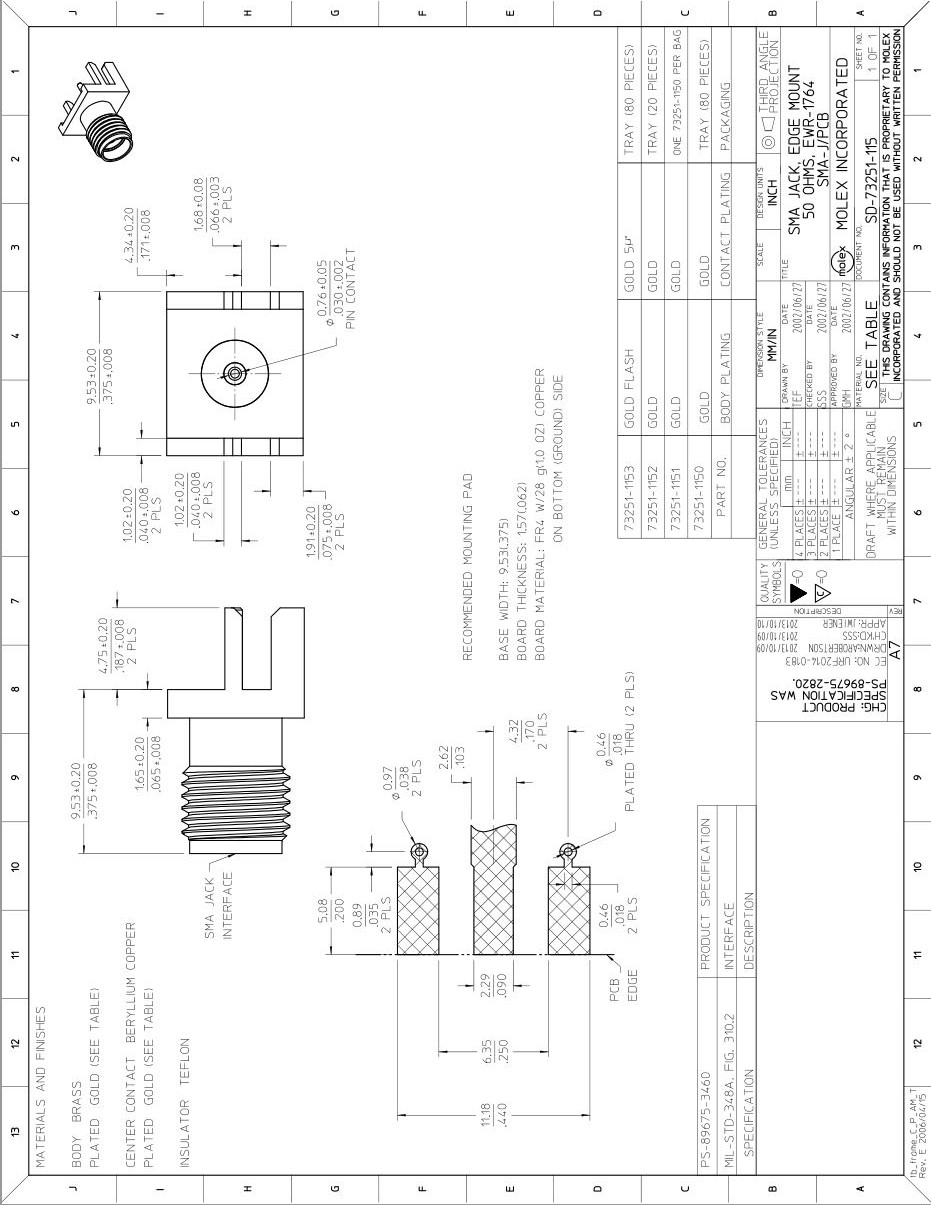
\includegraphics[width = .9\textwidth]{Tesis/Imagenes/Datos.JPG}
 		\captionof{figure}{Hoja de datos del jack SMD para antena de RF} 
	\label{Ap-jackRF}
    \end{center} 
\end{figure}

